\subsection{Creating Ansatzes}
\almarginpar{Which of the ansatze would be most useful to support QNN? Wouldn't RealAmplitudes be useful for "real" QNN implementation?}
We have chosen two ansatzes \textit{NLocal} and \textit{TwoLocal} from the Qiskit circuit library due to their wide usage in quantum machine learning.

An example of circuits generated by Qiskit is visualised in Figure \ref{Ansatz samples}.
By altering the repetition number and qubit number, we can generate different ansatz.
The circuit depth is the largest number of gate operations across all qubit registers in a circuit.
Furthermore, as the circuit high-level definition is translated into the gate set available on a given quantum machine, the circuit depth may significantly increase.
Obviously, as the ansatz repetition grows, the circuit depth also grows.
Figure \ref{Ansatz samples} further shows that for a fully entangled ansatz, the higher number of qubits also leads to deeper circuit.

\begin{figure}
    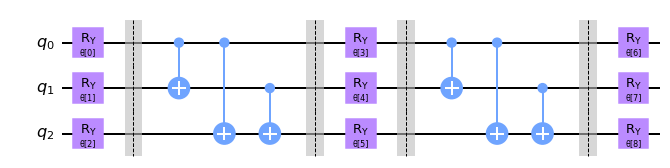
\includegraphics[width=\textwidth]{Artefact/Appendices/ansatz3-2.png}
    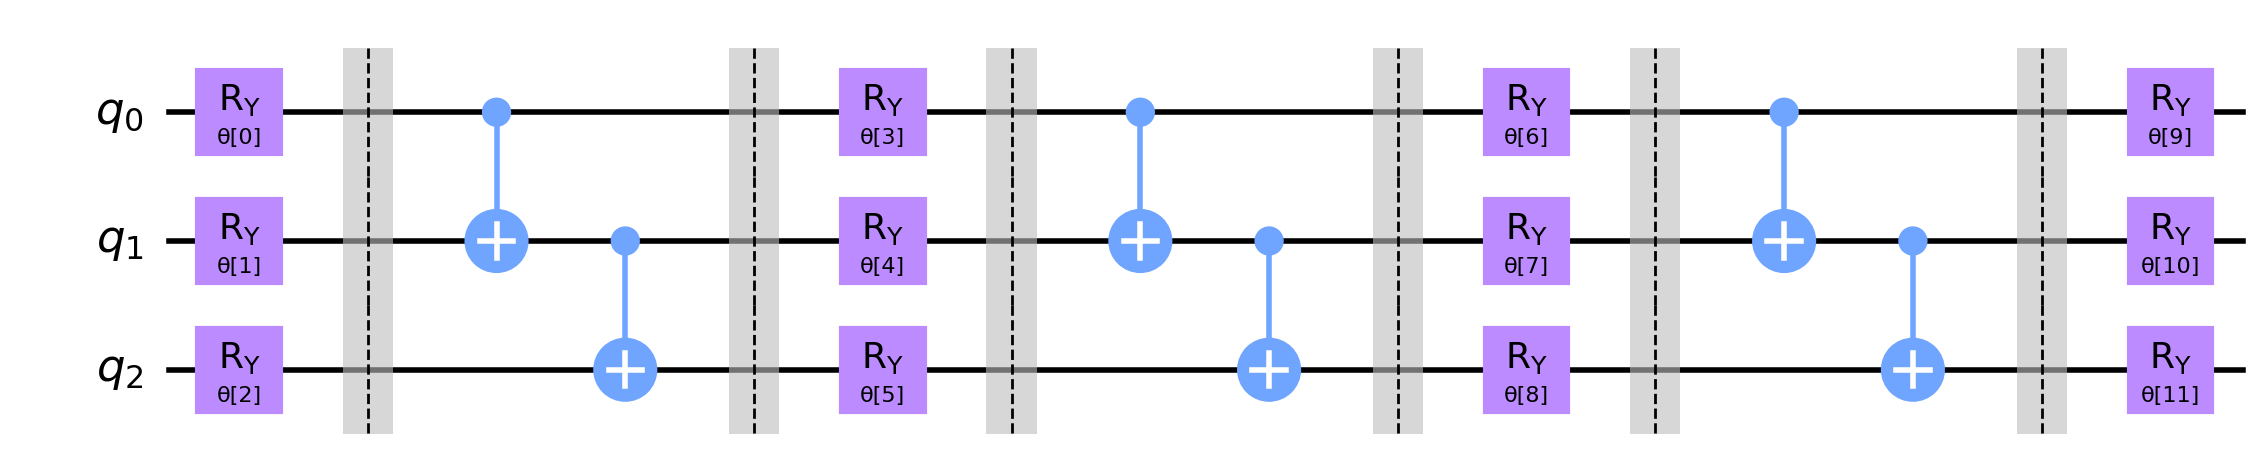
\includegraphics[width=\textwidth]{Artefact/Appendices/ansatz3-3.png}
    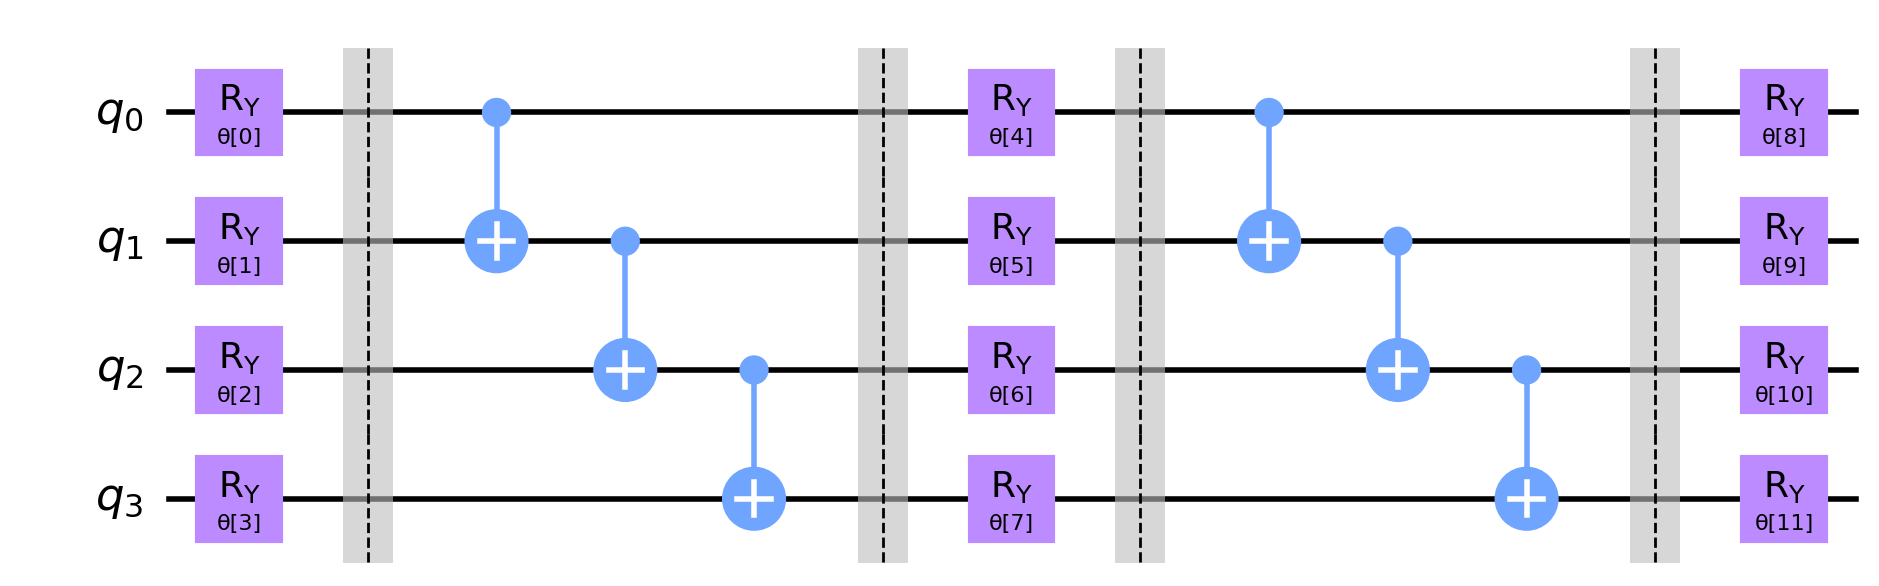
\includegraphics[width=\textwidth]{Artefact/Appendices/ansatz4-2.png}
    \caption{
        Samples of parameterised circuits generated by the Qiskit framework with 'full entanglement' option.
        The ansatz is a sequence of rotation layers and entanglement layers.
        Above: an ansatz of three qubits and two repetition layers.
        Middle: an ansatz of three qubits and three repetition layers.
        Below: an ansatz of four qubits and two repetition layers.
    }
    \label{Ansatz samples}
\end{figure}